\documentclass[xcolor=dvipsnames]{beamer}  % for hardcopy add 'trans'

\mode<presentation>
{
  \usetheme{Singapore}
  % or ...
  \setbeamercovered{transparent}
  % or whatever (possibly just delete it)
}

\usefonttheme{professionalfonts}

%%%%%%%%%%%%%%%%%%%%%% start my preamble %%%%%%%%%%%%%%%%%%%%%%
\renewcommand{\insertnavigation}[1]{}

%\pgfplotsset{compat=1.16}

\addtobeamertemplate{navigation symbols}{}{%
    \usebeamerfont{footline}%
    \usebeamercolor[fg]{footline}%
    \hspace{1em}%
    \insertframenumber/\inserttotalframenumber
}

\setbeamercolor{footline}{fg=blue}
\setbeamerfont{footline}{series=\bfseries}

\hypersetup{
    linkcolor=blue,
    colorlinks=true,
    filecolor=magenta,      % color of file links
    urlcolor=blue           % color of external links
}


%\pgfdeclareimage[height=1.0cm]{university-logo}{../qe-logo}
%\logo{\pgfuseimage{university-logo}}

%\addtobeamertemplate{headline}{}
%{%
%\begin{flushright}
%\begin{tikzpicture}[remember picture,overlay]
%\node [left ]{\includegraphics[width=0.5cm]{../tuxswatter2.png}};
%\end{tikzpicture}
%\end{flushright}
%\vskip -0.1cm
%} 


% algos
\usepackage{graphicx}
\usepackage{amsmath, amssymb, amsthm}
\usepackage{fancyvrb}
\usepackage{hyperref}
\usepackage{bbm}

%\usepackage{stix}
\usepackage{unicode-math}
\setmainfont{XITS}
\setmathfont{XITS Math}

% tikz
\usepackage{tikz}
\usepackage{tkz-graph}
\usepackage{tikz-cd}
\usetikzlibrary{positioning}
\usetikzlibrary{arrows}
\usetikzlibrary{calc}
\usetikzlibrary{intersections}
\usetikzlibrary{decorations}
\usepackage{pgf}
%\usepackage{pgfplots}



\usepackage{graphviz}

%\usepackage[usenames, dvipsnames]{color}


% nice inequalities
\renewcommand{\leq}{\leqslant}
\renewcommand{\geq}{\geqslant}


\setlength{\parskip}{1.5ex plus0.5ex minus0.5ex}
\setlength{\jot}{12pt} 

\usepackage[lined]{algorithm2e}


\definecolor{pale}{RGB}{235, 235, 235}
\definecolor{pale2}{RGB}{175,238,238}
\definecolor{turquois4}{RGB}{0,134,139}
\definecolor{DarkOrange1}{RGB}{255,127,0}

\newcommand{\emp}[1]{\textcolor{DarkOrange1}{\bf #1}}
\newcommand{\newtopic}[1]{\textcolor{Green}{\Large \bf #1}}
\newcommand{\navy}[1]{\textcolor{blue}{\bf #1}}
\newcommand{\blue}[1]{\textcolor{turquois4}{#1}}
\newcommand{\red}[1]{\textcolor{red}{#1}}

% Minted
\definecolor{bg}{rgb}{0.95,0.95,0.95}
\usepackage{minted}
\usemintedstyle{friendly}
\newminted{python}{mathescape,frame=lines,framesep=4mm,bgcolor=bg}
\newminted{ipython}{mathescape,frame=lines,framesep=4mm,bgcolor=bg}
\newminted{julia}{mathescape,frame=lines,framesep=4mm,bgcolor=bg}
\newminted{c}{mathescape,frame=lines,framesep=4mm,bgcolor=bg}
\renewcommand{\theFancyVerbLine}{\sffamily
    \textcolor[rgb]{0.5,0.5,1.0}{\scriptsize {\arabic{FancyVerbLine}}}}

\newcommand{\ess}{ \textrm{{\sc ess}} }
\newcommand{\tss}{ \textrm{{\sc tss}} }
\newcommand{\ssr}{ \textrm{{\sc ssr}} }

\newcommand{\Fact}{\textcolor{Brown}{\bf Fact. }}
\newcommand{\Facts}{\textcolor{Brown}{\bf Facts }}
\newcommand{\keya}{\textcolor{turquois4}{\bf Key Idea. }}
\newcommand{\Factnodot}{\textcolor{Brown}{\bf Fact }}
\newcommand{\Eg}{\textcolor{ForestGreen}{Example. }}
\newcommand{\Egs}{\textcolor{ForestGreen}{Examples. }}
\newcommand{\Ex}{{\bf Ex. }}

\newcommand{\argmax}{\operatornamewithlimits{argmax}}
\newcommand{\argmin}{\operatornamewithlimits{argmin}}

\DeclareMathOperator{\cl}{cl}
\DeclareMathOperator{\gr}{gr}
\DeclareMathOperator{\interior}{int}
\DeclareMathOperator{\Prob}{Prob}
\DeclareMathOperator{\kernel}{ker}
\DeclareMathOperator{\diag}{diag}
\DeclareMathOperator{\sgn}{sgn}
\DeclareMathOperator{\determinant}{det}
\DeclareMathOperator{\trace}{trace}
\DeclareMathOperator{\Span}{span}
\DeclareMathOperator{\rank}{rank}
\DeclareMathOperator{\cov}{cov}
\DeclareMathOperator{\corr}{corr}
\DeclareMathOperator{\range}{rng}
\DeclareMathOperator{\var}{var}
\DeclareMathOperator{\mse}{mse}
\DeclareMathOperator{\se}{se}
\DeclareMathOperator{\row}{row}
\DeclareMathOperator{\col}{col}
\DeclareMathOperator{\dimension}{dim}
\DeclareMathOperator{\fracpart}{frac}
\DeclareMathOperator{\proj}{proj}

% mics short cuts and symbols
\newcommand{\st}{\ensuremath{\ \mathrm{s.t.}\ }}
\newcommand{\setntn}[2]{ \{ #1 : #2 \} }
\newcommand{\cf}[1]{ \lstinline|#1| }
\newcommand{\fore}{\therefore \quad}
\newcommand{\tod}{\stackrel { d } {\to} }
\newcommand{\toprob}{\stackrel { p } {\to} }
\newcommand{\toms}{\stackrel { ms } {\to} }
\newcommand{\eqdist}{\stackrel {\mathscr{D}}{=} }
\newcommand{\iidsim}{\stackrel {\textrm{ {\sc iid }}} {\sim} }
\newcommand{\1}{\mathbbm 1}
\newcommand{\given}{\, | \,}
\newcommand{\la}{\langle}
\newcommand{\ra}{\rangle}
\newcommand{\lra}{\leftrightarrow}

\providecommand{\inner}[1]{\left\langle{#1}\right\rangle}

% d for integrals
\newcommand*\diff{\mathop{}\!\mathrm{d}}

\newcommand{\RR}{\mathbbm R}
\newcommand{\NN}{\mathbbm N}
\newcommand{\PP}{\mathbbm P}
\newcommand{\DD}{\mathbbm D}
\newcommand{\EE}{\mathbbm E}
\newcommand{\GG}{\mathbbm G}
\newcommand{\WW}{\mathbbm W}
\newcommand{\ZZ}{\mathbbm Z}
\newcommand{\QQ}{\mathbbm Q}


\newcommand{\XX}{\mathsf X}
\newcommand{\YY}{\mathsf Y}

\newcommand{\fF}{\mathscr F}
\newcommand{\sS}{\mathscr S}
\newcommand{\jJ}{\mathscr J}
\newcommand{\cC}{\mathscr C}
\newcommand{\aA}{\mathscr A}
\newcommand{\bB}{\mathscr B}
\newcommand{\gG}{\mathscr G}
\newcommand{\hH}{\mathcal H}
\newcommand{\nN}{\mathscr N}
\newcommand{\dD}{\mathscr D}
\newcommand{\oO}{\mathscr O}
\newcommand{\pP}{\mathscr P}
\newcommand{\lL}{\mathscr L}

\newcommand{\rR}{\mathcal R}
\newcommand{\mM}{\mathcal M}







\begin{document}

%\begin{frame}
%  \titlepage
%\end{frame}


\begin{frame}
    
    \begin{center}
        \navy{\Large{Stochastic Approximation}}

        
        \vspace{2em}
        John Stachurski 

        \vspace{1em}
        \vspace{1em}
        %\today{}
        \texttt{\today}

    \end{center}

\end{frame}

\begin{frame}
    \frametitle{Overview}
    
    \begin{itemize}
        \item Fixed point iteration
            \vspace{0.5em}
        \item Stochastic approximation
            \vspace{0.5em}
        \item Examples
    \end{itemize}

\end{frame}


\begin{frame}
    \frametitle{Fixed point iteration}

    Let 
    %
    \begin{itemize}
        \item $T \colon \Theta \to \Theta$ be a contraction map of modulus $\beta$
        \item $\Theta$ be a closed subset of $\RR^n$
    \end{itemize}

    \vspace{0.5em}
    \vspace{0.5em}
    We know that $T^k \theta \to \bar \theta$ as $k \to \infty$ where $\bar
    \theta$ is the
    unique fixed point

    \vspace{0.5em}
    Alternatively, we can iterate on the damped sequence
    %
    \begin{align*}
        \theta_{k+1} 
        & = (1-\alpha) \theta_k + \alpha T \theta_k
        \\
        & =  \theta_k + \alpha (T \theta_k - \theta_k)
    \end{align*}

    \begin{itemize}
        \item $\alpha \in (0,1)$
    \end{itemize}

\end{frame}




\begin{frame}

    To see that the damped sequence converges, let
    %
    \begin{equation*}
        F\theta = \theta + \alpha (T\theta - \theta)
    \end{equation*}

    Then
    %
    \begin{equation*}
        F \bar \theta 
        = \bar \theta + \alpha (T \bar \theta - \bar \theta)
        = \bar \theta
    \end{equation*}

    and

    \begin{equation*}
        \| F\theta - F\theta'\|
        \leq (1-\alpha)\|\theta - \theta'\| + \alpha \| T\theta - T\theta'\|
        \leq (1-\alpha + \alpha \beta)\| \theta - \theta'\|
    \end{equation*}

    Note 
    %
    \begin{equation*}
        1-\alpha + \alpha \beta < 1
        \iff \beta < 1
    \end{equation*}
    
\end{frame}

\begin{frame}
    Sometimes damped iteration is faster

    \vspace{1em}

    This tends to be true when there are oscillations

    \vspace{1em}
    \vspace{1em}
    For example, let's ordinary and damped iteration it with
    \vspace{1em}

    \begin{equation*}
        T = A = 
        \begin{pmatrix}
            0.5 & 0.6 \\
            0.4 & -0.7
        \end{pmatrix}
        \quad \text{and} \quad
        \alpha = 0.7
    \end{equation*}

    The fixed point is 

    \begin{equation*}
        \bar \theta = 
        \begin{pmatrix}
            0 \\
            0
        \end{pmatrix}
    \end{equation*}

\end{frame}

\begin{frame}

    \begin{figure}
        \centering
        \scalebox{0.5}{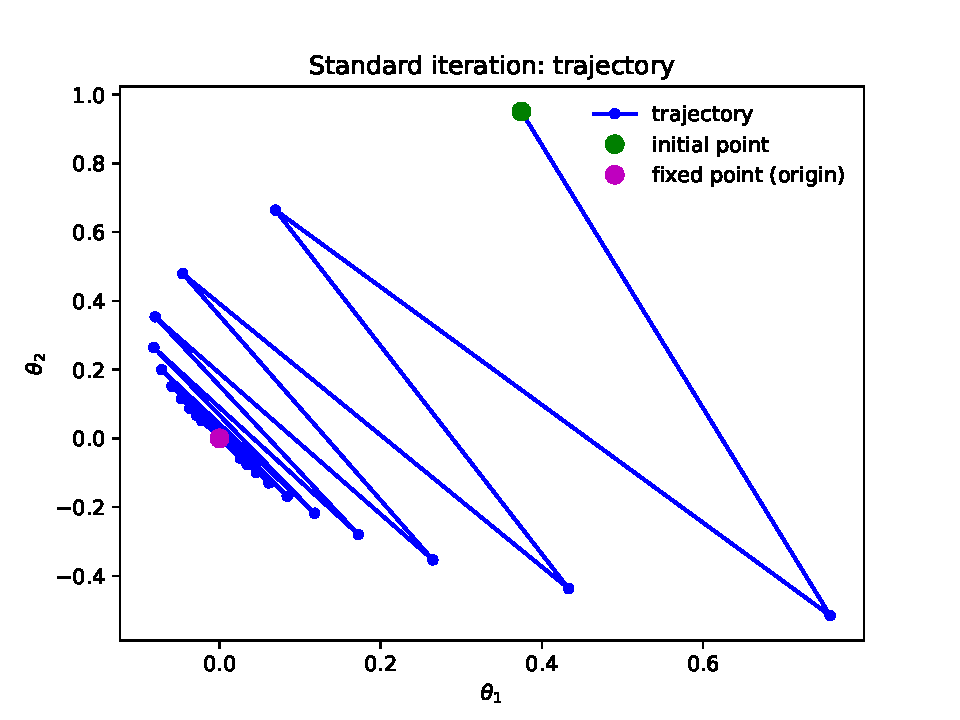
\includegraphics[trim={0cm 0cm 0cm 0cm},clip]{damped_1.pdf}}
    \end{figure}
    
\end{frame}

\begin{frame}

    \begin{figure}
        \centering
        \scalebox{0.5}{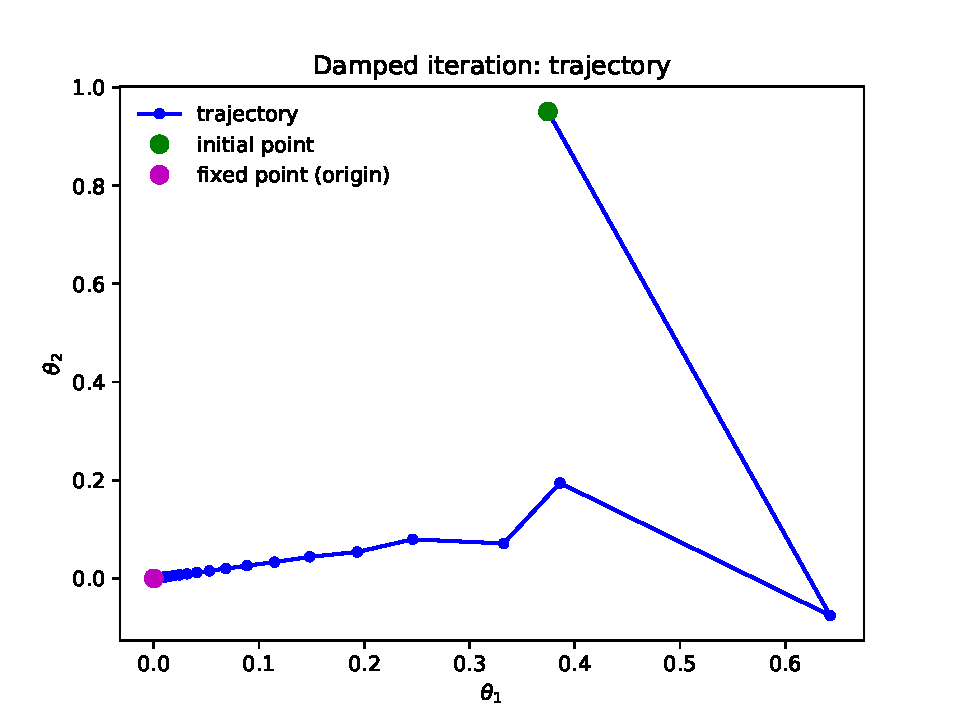
\includegraphics[trim={0cm 0cm 0cm 0cm},clip]{damped_2.pdf}}
    \end{figure}
    
\end{frame}


\begin{frame}

    \begin{figure}
        \centering
        \scalebox{0.5}{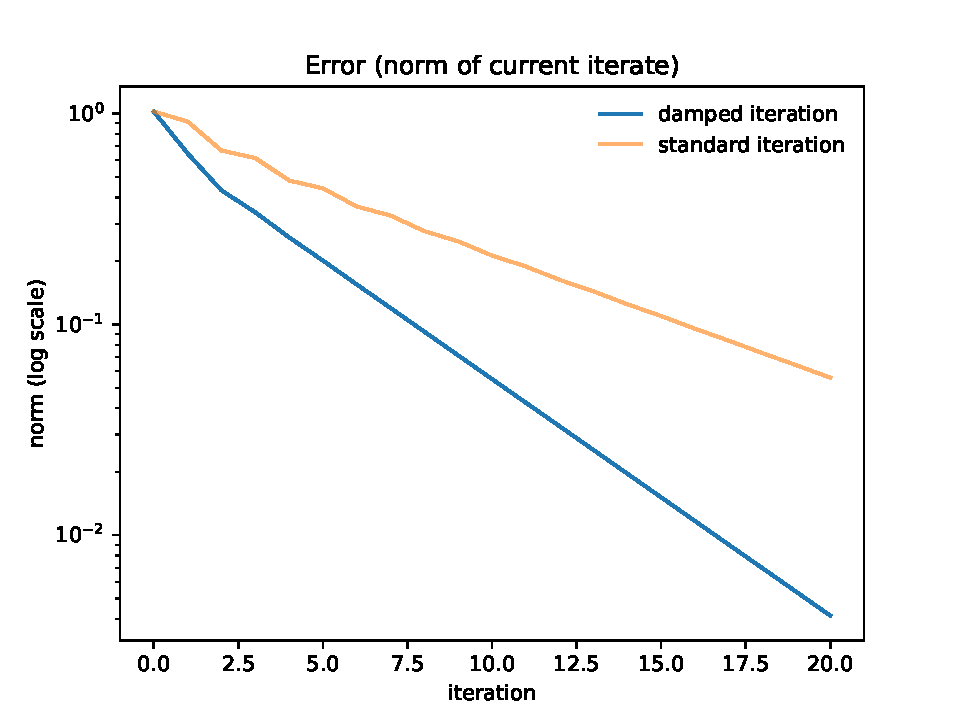
\includegraphics[trim={0cm 0cm 0cm 0cm},clip]{damped_3.pdf}}
    \end{figure}
    
\end{frame}

\begin{frame}
    \frametitle{Stochastic Approximation}

    Suppose $T$ is a map with fixed point $\bar \theta = T \bar \theta$

    We can only evaluate $T$ with noise:
    %
    \begin{center}
        input $\theta$ and receive $T \theta + W$ 
    \end{center}

    \begin{itemize}
        \item $(W_k)$ is a random (vector-valued) sequence 
        \item We cannot observe $W_k$, only $T \theta + W_k$
    \end{itemize}

    Robbins--Monro algorithm to compute the fixed point $\bar \theta$:
    %
    \begin{equation*}
        \theta_{k+1} 
        = \theta_k + \alpha_k [ T \theta_k + W_k - \theta_k ]
    \end{equation*}

    \begin{itemize}
        \item $(\alpha_k)$ is a sequence in $(0,1)$
    \end{itemize}

\end{frame}


\begin{frame}
    
    Side-by-side comparison:

    \vspace{1em}

    Here's damped iteration:

    \begin{equation*}
        \theta_{k+1} = \theta_k + \alpha (T \theta_k - \theta_k)
    \end{equation*}

    \vspace{1em}
    \vspace{1em}

    This is Robbins--Monro 
    %
    \begin{equation*}
        \theta_{k+1} 
        = \theta_k + \alpha_k ( T \theta_k + W_k - \theta_k )
    \end{equation*}

\end{frame}


\begin{frame}
    
    By our earlier analysis, $\theta_k \to \bar \theta$ if $W_k \equiv 0$ and
    $\alpha_k \equiv \alpha$

    \vspace{0.5em}
    More generally, \cite{tsitsiklis1994asynchronous} proves that if:
    %
    \begin{itemize}
        \item $T$ is an order-preserving contraction map with fixed
            point $\bar \theta$
            \vspace{0.5em}
        \item $\EE [W_{k+1} \given \fF_k] = 0$ for all $k \geq 0$
            \vspace{0.5em}
        \item $\sum_{k \geq 0} \alpha_k = \infty$ and $\sum_{k \geq 0} \alpha_k^2 < \infty$
            \vspace{0.5em}
        \item some other technical assumptions,
    \end{itemize}
    %
    then 
    %
    \begin{center}
        $\theta_k \to \bar \theta$ with probability one
    \end{center}

\end{frame}


\begin{frame}
    \frametitle{Example: Asset Pricing}

    The value of an asset is given by
    %
    \begin{equation*}
        V_t = \EE_t M_{t+1} [V_{t+1} + D_{t+1}]
    \end{equation*}

    Assume that 
    %
    \begin{itemize}
        \item $(X_t)$ is $P$-Markov on finite set $\XX$
        \item $M_{t+1} = m(X_{t+1})$ for all $t$
        \item $D_{t+1} = d(X_{t+1})$ for all $t$
    \end{itemize}

    (This is a version of a standard Lucas tree model.)

\end{frame}

\begin{frame}
    
    Then the solution has the form $V_t = v(X_t)$ where $v$ solves

    \begin{equation*}
        v(x) = \sum_{x'} m(x') [v(x') + d(x')]  P(x,x') 
    \end{equation*}

    With 
    %
    \begin{equation*}
        (Kf)(x) \coloneq \sum_{x'} m(x') f(x')  P(x,x') 
        \quad \text{and} \quad
        b(x) \coloneq Kd
    \end{equation*}
    %
    we can write the equation as 
    %
    \begin{equation*}
        v = Tv 
        \quad \text{where} \quad
        Tv \coloneq Kv + b
    \end{equation*}

    The solution has the form
    %
    \begin{equation*}
        v^* = (I - K)^{-1} b
    \end{equation*}

\end{frame}

\begin{frame}
    
    We can also compute $v^*$ by stochastic approximation

    Consider the sequence generated by

    \begin{algorithm}
        \DontPrintSemicolon
        foo
        % \For{$x \in \XX$}
        % {
        %     $v_{k+1}(x) \rightarrow v_k(x) + \alpha_k(m(Y)v(Y) + d(Y) - v_k(x))$
        % }
    \end{algorithm}

    %

\end{frame}


\begin{frame}[allowframebreaks]
    \frametitle{References}

    \bibliographystyle{amsalpha}

    \bibliography{../main.bib}

\end{frame}


\end{document}
